%!TEX TS-program = xelatex
\documentclass{EdipyLabs} % Custom class provided for EDIPY labs, by Christos Dalamagkas (cdalamagkas@gmail.com)
\SetLabNumber{2α}
\SetLabTitle{Διευθέτηση δρομολογητή}
\SetAuthor{Χρήστος Δαλαμάγκας}
\SetLabDescription{Αρχιτεκτονική δρομολογητών, πίνακας δρομολόγησης, Υλοποίηση τοπολογίας, βασική παραμετροποίηση δρομολογητών και διεπαφών, στατική δρομολόγηση, προεπιλεγμένη πύλη δικτύου.}
\SetLabPrerequisites{Εργαστηριακό φυλλάδιο 1α (Εισαγωγή στο Cisco IOS).}

\begin{document}

\Initialize

\section*{Εισαγωγή}
Αντικείμενο του παρόντος εργαστηριακού φυλλαδίου αποτελεί η επισκόπηση της λειτουργίας των δρομολογητών, η διερεύνηση βασικών εντολών διαχείρισης δρομολογητών Cisco, καθώς και η εισαγωγή σε βασικές αρχές σχεδίασης δικτύων, όπως η σχεδίαση και υλοποίηση μιας τοπολογίας. Στο πλαίσιο της εργαστηριακής άσκησης θα υλοποιήσετε τη δικτυακή τοπολογία που φαίνεται στο σχήμα \ref{topology1} και θα πραγματοποιήσετε δοκιμές συνδεσιμότητας σε αυτήν.

\begin{figure}[H]
	\centering
	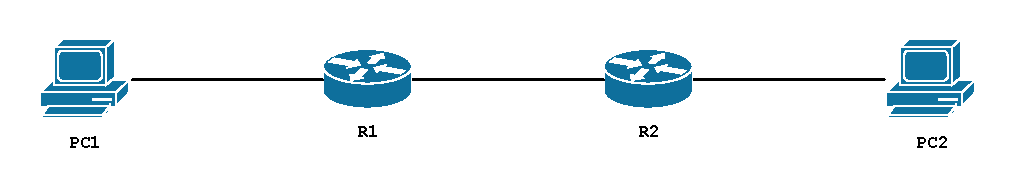
\includegraphics[width=\linewidth]{topology}
	\caption{Βασικό σχέδιο της δικτυακής τοπολογίας προς υλοποίηση.}\label{topology1}
\end{figure}

Για την υλοποίηση της τοπολογίας θα χρειαστείτε τις εξής συσκευές:
\begin{itemize}
	\item x2 δρομολογητές Cisco 2921
	\item x2 υπολογιστές
\end{itemize}

\section{Θεωρητικό υπόβαθρο}

Ο δρομολογητής (router) είναι μια δικτυακή συσκευή που προωθεί πακέτα μεταξύ διαφορετικών δικτύων. Ο ρόλος του στην προώθηση πακέτων είναι θεμελιώδης, διότι το σύνολο των δρομολογητών που διασυνδέονται μεταξύ τους κατασκευάζουν το γνωστό Διαδίκτυο. Το γεγονός ότι ο δρομολογητής διασυνδέει πολλαπλά δίκτυα σημαίνει ότι διαθέτει πολλές διεπαφές (nterfaces), με κάθε μια εξ αυτών να ανήκει σε διαφορετικό δίκτυο. Η χρησιμότητα των δρομολογητών συνοψίζεται στα εξής σημεία:
\begin{itemize}
	\item Διασυνδέουν δίκτυα.
	\item Καθορίζουν τη βέλτιστη διαδρομή για να στείλουν πακέτα.
	\item Προωθούν πακέτα προς τον προορισμό τους.
\end{itemize}

Δεν είναι υπερβολικό να υποστηρίξει κάποιος ότι η λειτουργία του Διαδικτύου στηρίζεται στην απόφαση του δρομολογητή για τη διεπαφή προς την οποία θα προωθήσει ένα πακέτο, με σκοπό αυτό να φτάσει στον προορισμό του. Η απόφαση της προώθησης λαμβάνεται με τη χρήση του \textbf{πίνακα δρομολόγησης} (routing table). Ο πίνακας δρομολόγησης είναι μια δομή δεδομένων, η οποία αποθηκεύεται στη μνήμη RAM και αντιστοιχίζει δίκτυα προορισμού με διεπαφές εξόδου ή διευθύνσεις IP επόμενου άλματος.

Πιο αναλυτικά, όταν ένα πλαίσιο εισέρχεται σε μια διεπαφή ενός δρομολογητή, ο δρομολογητής καταστρέφει την επικεφαλίδα του στρώματος ζεύξης δεδομένων, εξάγει τη διεύθυνση IP προορισμού του πακέτου και ελέγχει αν αυτή ανήκει σε κάποιο δίκτυο του πίνακα δρομολόγησης. Ο έλεγχος γίνεται με λογικό AND της διεύθυνσης IP προορισμού με τη μάσκα υποδικτύου του κάθε δικτύου του πίνακα. Αν βρεθεί ότι η διεύθυνση IP προορισμού ανήκει σε κάποιο δίκτυο του πίνακα, τότε το πακέτο προωθείται στην αντίστοιχη διεπαφή. Αν δεν βρεθεί αντιστοιχία, τότε το πακέτο προωθείται στην πύλη δικτύου (gateway), αλλιώς απορρίπτεται. Ο πίνακας δρομολόγησης εμφανίζεται με την εντολή \texttt{show ip route}:

\begin{CommandBox}
R1#`\textbf{show ip route | begin Gateway}`
Gateway of last resort is not set

     172.16.0.0/16 is variably subnetted, 2 subnets, 2 masks
C       172.16.1.0/30 is directly connected, GigabitEthernet0/1
L       172.16.1.1/32 is directly connected, GigabitEthernet0/1
     192.168.10.0/24 is variably subnetted, 2 subnets, 2 masks
C       192.168.10.0/24 is directly connected, GigabitEthernet0/0
L       192.168.10.1/32 is directly connected, GigabitEthernet0/0
R1#
\end{CommandBox}

Τα δίκτυα που περιλαμβάνονται σε έναν πίνακα δρομολόγησης ανήκουν σε μια από τις εξής δυο κατηγορίες:
\begin{itemize}
	\item \textbf{Απευθείας συνδεδεμένα} (directly connected): Είναι τα δίκτυα με τα οποία ο δρομολογητής συνδέεται απευθείας μέσω των διεπαφών του. Στο σχήμα \ref{fig:table1} απεικονίζεται η μορφή των εν λόγω καταχωρήσεων στον πίνακα δρομολόγησης του Cisco IOS. Το C στην πηγή καταχώρησης αφορά την ταυτότητα του απευθείας συνδεδεμένου δικτύου, ενώ η καταχώριση L, που περιλαμβάνεται στις νεώτερες εκδόσεις του Cisco IOS, υποδηλώνει την IP που διαθέτει η διεπαφή του δρομολογητή στο αντίστοιχο δίκτυο. Όταν ο διαχειριστής αναθέτει διεύθυνση IP σε μια διεπαφή και την ενεργοποιεί, τότε δημιουργούνται αυτόματα δυο αντίστοιχες καταχωρήσεις L και C στον πίνακα δρομολόγησης.
	
	\begin{figure}[ht]
		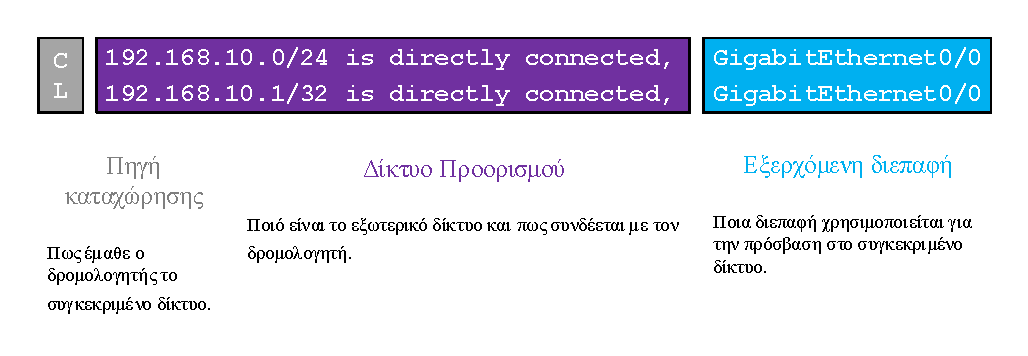
\includegraphics[width=\linewidth]{table1}
		\caption{H μορφή καταχώρησης απευθείας συνδεδεμένων δικτύων στον πίνακα δρομολόγησης του Cisco IOS.}\label{fig:table1}
	\end{figure}
	
	\item \textbf{Απομακρυσμένα δίκτυα} (remote networks): Είναι τα δίκτυα με τα οποία ο δρομολογητής δεν συνδέεται απευθείας αλλά μέσω κάποιου γειτονικού δρομολογητή. Οι καταχωρίσεις αυτές μπορούν να προέλθουν είτε \textbf{στατικά}, από καταχωρήσεις του διαχειριστή δικτύου, είτε \textbf{δυναμικά}, από κάποιο πρωτόκολλο δυναμικής δρομολόγησης.
	
	\begin{figure}[ht]
		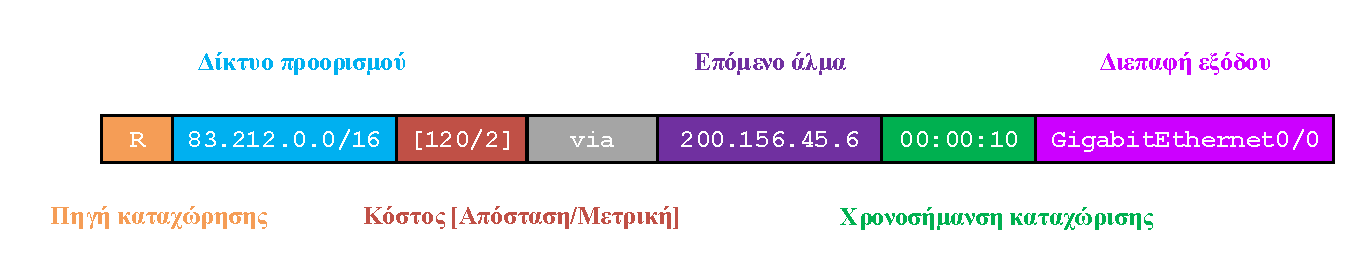
\includegraphics[width=\linewidth]{routing-table}
		\caption{H μορφή καταχώρησης απομακρυσμένων δικτύων στον πίνακα δρομολόγησης του Cisco IOS.}\label{fig:routing-table}
	\end{figure}
	
	Στο σχήμα \ref{fig:routing-table} απεικονίζεται μια δυναμική καταχώριση στον πίνακα δρομολόγησης, όπως αυτή εμφανίζεται στο Cisco IOS. Μια τέτοια καταχώριση αποτελείται από τις εξής πληροφορίες:
	\begin{itemize}
		\item \textbf{Πηγή καταχώρισης}: Το πρωτόκολλο από το οποίο προέρχεται η καταχώριση. To R υποδεικνύει το πρωτόκολλο RIP. Όλες οι ενδείξεις εμφανίζονται με την εντολή \texttt{show ip route}.
		\item \textbf{Δίκτυο προορισμού}: To απομακρυσμένο δίκτυο το οποίο αφορά η καταχώριση.
		\item \textbf{Κόστος}: Το κόστος της διαδρομής, όπως υπολογίστηκε από το πρωτόκολλο δυναμικής δρομολόγησης. Η (διαχειριστική) απόσταση προσδιορίζει την αξιοπιστία του πρωτοκόλλου, ενώ η μετρική λαμβάνεται υπόψιν όταν ο δρομολογητής έχει να διαλέξει από διαδρομές με την ίδια απόσταση.
		\item \textbf{Επόμενο άλμα}: Η διεύθυνση IP του δρομολογητή, στον οποίο πρέπει να προωθηθεί το πακέτο. Ο δρομολογητής επόμενου άλματος πρέπει να ανήκει σε δίκτυο που είναι απευθείας συνδεδεμένο με τον δρομολογητή, στον οποίο υπάρχει αυτή η καταχώριση. 
		\item \textbf{Χρονοσήμανση} (timestamp): Πριν από πόσο χρονικό διάστημα έγινε η τελευταία ενημέρωση της καταχώρισης.
		\item \textbf{Διεπαφή εξόδου}: Η διεπαφή προς την οποία πρέπει να προωθηθεί το πακέτο.
	\end{itemize}
\end{itemize}

Στην περίπτωση που κατά την αναζήτηση στον πίνακα δρομολόγησης μια διεύθυνση IP προορισμού ταυτίζεται με περισσότερες διαδρομές, τότε λαμβάνεται υπόψιν αυτή με το μεγαλύτερο πρόθεμα (longest prefix match). Για παράδειγμα, αν ένα πακέτο με διεύθυνση προορισμού 192.168.1.5 ταυτίζεται με τις καταχωρίσεις 192.168.0.0/16, 192.168.1.0/24 και 192.168.1.0/28 ενός πίνακα δρομολόγησης, τότε επιλέγεται αυτή με το μεγαλύτερο πρόθεμα, δηλαδή η 192.168.1.0/28.

\begin{figure}[ht]
	\centering
	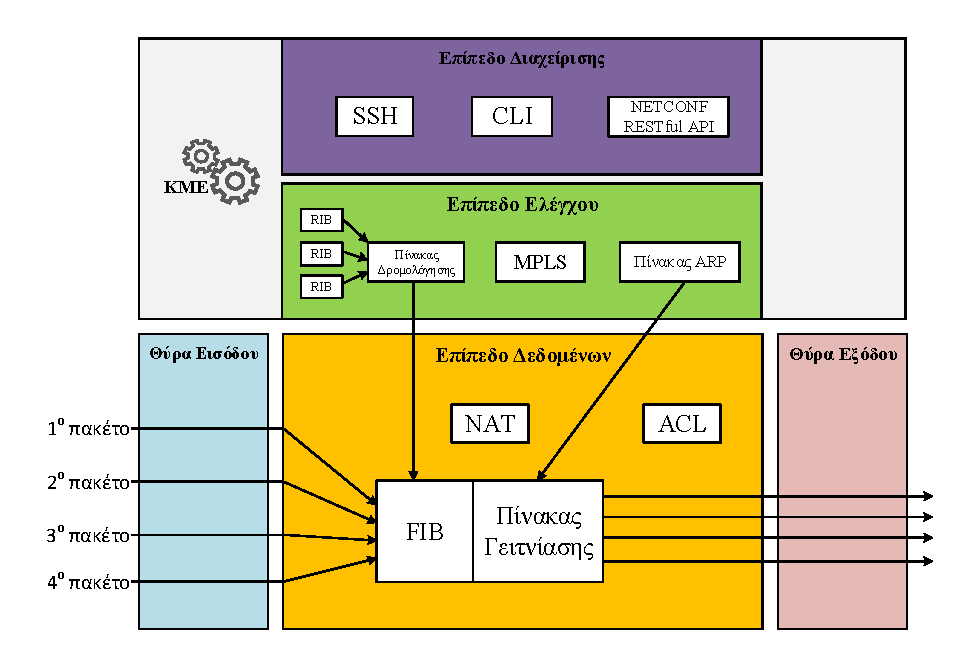
\includegraphics[width=\linewidth]{planes}
	\caption{Η γενική άποψη της αρχιτεκτονικής ενός δρομολογητή.}\label{fig:planes}
\end{figure}

Ο πίνακας δρομολόγησης αποτελεί κομμάτι μιας πιο αφηρημένης αρχιτεκτονικής που ακολουθούν οι σύγχρονοι δρομολογητές, η οποία απεικονίζεται στο σχήμα \ref{fig:planes}. Οι διάφορες λειτουργίες και τα πρωτόκολλα που υποστηρίζει ένας δρομολογητής μοιράζονται μεταξύ του \textbf{Επιπέδου Διαχείρισης} (Management Plane), του \textbf{Επιπέδου Ελέγχου} (Control Plane) και του \textbf{Επιπέδου Δεδομένων} (Data Plane). 

Το \textbf{επίπεδο διαχείρισης} παρέχει όλες εκείνες τις διεπαφές λογισμικού και τις υπηρεσίες που χρησιμεύουν στην απομακρυσμένη και μη διαχείριση της συσκευής. Στο επίπεδο αυτό συμπεριλαμβάνονται κατά κύριο λόγο πρωτόκολλα και υπηρεσίες του επιπέδου εφαμρογών, όπως το SSH, καθώς και εφαρμογές διαχείρισης στα πρότυπα SDN (Software Defined Networking), όπως το NETCONF και το RESTCONF.

Το \textbf{επίπεδο ελέγχου}, μεταξύ πολλών αρμοδιοτήτων, καταγράφει τη δικτυακή τοπολογία, διαχειρίζεται τους πίνακες δρομολόγησης και διατηρεί τον πίνακα ARP που αντιστοιχίζει διευθύνσεις MAC με αντίστοιχες IP. Στο επίπεδο αυτό, κάθε πρωτόκολλο δρομολόγησης διατηρεί μια τοπική βάση δεδομένων, που αποκαλείται \textbf{Βάση Πληροφοριών Δρομολόγησης} (Routing Information Base - RIB), η οποία περιλαμβάνει τις διαδρομές που το συγκεκριμένο πρωτόκολλο έχει καταγράψει από την τοπολογία. Η τελική καλύτερη διαδρομή που επιλέγεται για κάθε προορισμό εγκαθίσταται από το επίπεδο ελέγχου στο καθολικό RIB, δηλαδή τον πίνακα δρομολόγησης, ο οποίος εμφανίζεται στο Cisco IOS με την εντολή \texttt{show ip route} και στο RouterOS με την εντολή \texttt{/ip route print}. Η διαδρομή εκείνη που τελικά εγκαθίσταται στον πίνακα δρομολόγησης αποκαλείται \textbf{ενεργή} διαδρομή.

Το \textbf{επίπεδο δεδομένων} εστιάζει στην επιταχυνόμενη προώθηση πακέτων μέσω ειδικά σχεδιασμένων κυκλωμάτων (Application-specific integrated circuit - ASIC), καθώς και σε εφαρμογές που μπορούν να επιταχυνθούν μέσω υλικού, όπως το NAT, οι λίστες ελέγχου (ACL) και τα τείχη ασφαλείας (firewall). Βασικό χαρακτηριστικό του επιπέδου είναι πως, σε αντίθεση με τα επίπεδα διαχείρισης και ελέγχου, δεν απασχολεί την Κεντρική Μονάδα Επεξεργασίας (ΚΜΕ), αλλά ειδικά προορισμένους επεξεργαστικούς πόρους. Σημαντικό τμήμα του επιπέδου δεδομένων είναι η \textbf{Βάση Πληροφοριών Προώθησης} (Forward Information Base - FIB), η οποία αντανακλά τα περιεχόμενα του πίνακα δρομολόγησης και κατ' ελάχιστον αντιστοιχίζει μια διεύθυνση IP επόμενου άλματος συγκεκριμένου προθέματος με μια διεπαφή εξόδου (\href{https://tools.ietf.org/html/rfc1812}{RFC 1812}). 

Αν και η FIB σχεδιάστηκε με σκοπό να μην απασχολείται η ΚΜΕ κατά τη διαδικασία προώθησης πακέτων, αυτό δεν γίνεται πάντα εφικτό. Στην περίπτωση που μια καταχώριση του πίνακα δρομολόγησης περιέχει μόνο τη διεύθυνση IP επόμενου άλματος, ο δρομολογητής πρέπει να αναζητήσει και την IP επόμενου άλματος στον πίνακα ώστε να εξάγει τη διεπαφή εξόδου και τις απαραίτητες πληροφορίες στρώματος ζεύξης δεδομένων. Η διπλή αυτή αναζήτηση στον πίνακα δρομολόγησης ονομάζεται αναδρομική (recursive lookup).

Την ανάγκη για αναδρομικές αναζητήσεις εξαλείφει η τεχνολογία \textbf{Cisco Express Forwarding} (CEF), η οποία επιταχύνει σημαντικά τη διαδικασία προώθησης πακέτων με την προσθήκη του πίνακα γειτνίασης (adjacency table), ο οποίος αντανακλά τα περιεχόμενα του πίνακα ARP από το επιπέδου ελέγχου, και περιέχει πληροφορίες στρώματος ζεύξης δεδομένων για τους γειτονικούς προορισμούς, ώστε τα πλαίσια να κατασκευάζονται άμεσα, χωρίς την ανάγκη για πρόσθετες αναζητήσεις.

\newpage

\section{Αναλυτική σχεδίαση τοπολογίας}
Πρώτο βήμα για την υλοποίηση μιας δικτυακής τοπολογίας αποτελεί η αναλυτική της σχεδίαση, η οποία περιλαμβάνει τις εξής ενέργειες:
\begin{itemize}
	\item Αναγνώριση των δικτύων, από τα οποία αποτελείται η τοπολογία.
	\item Διευθυνσιοδότηση των δικτύων και των επιμέρους συσκευών. Θα πρέπει να λάβετε υπόψιν το έγγραφο \href{https://tools.ietf.org/html/rfc1918}{RFC 1918}, αν σχεδιάζετε ιδιωτικά LAN.
	\item Επιλογή των διεπαφών, στις οποίες θα αντιστοιχιστούν τα δίκτυα του κάθε δρομολογητή.
\end{itemize}

Η γραφική αναπαράσταση της τοπολογίας της εργαστηριακής άσκησης απεικονίζεται στο σχήμα \ref{topology2} και το αντίστοιχο σχήμα διευθυνσιοδότησης στον πίνακα \ref{tab:addr}. Όπως φαίνεται στο σχήμα, η τοπολογία αποτελείται από τρία δίκτυα (ή τομείς ευρυεκπομπής):\textbf{192.168.10.0/24}, \textbf{172.16.1.0/30} και \textbf{192.168.20.0/24}. Κατά τη συνήθη πρακτική, στον δρομολογητή του πρώτου και του τρίτου δικτύου έχει ανατεθεί η πρώτη ωφέλιμη και στον υπολογιστή του καθενός η δεύτερη ωφέλιμη διεύθυνση IP.

\begin{figure}[ht]
	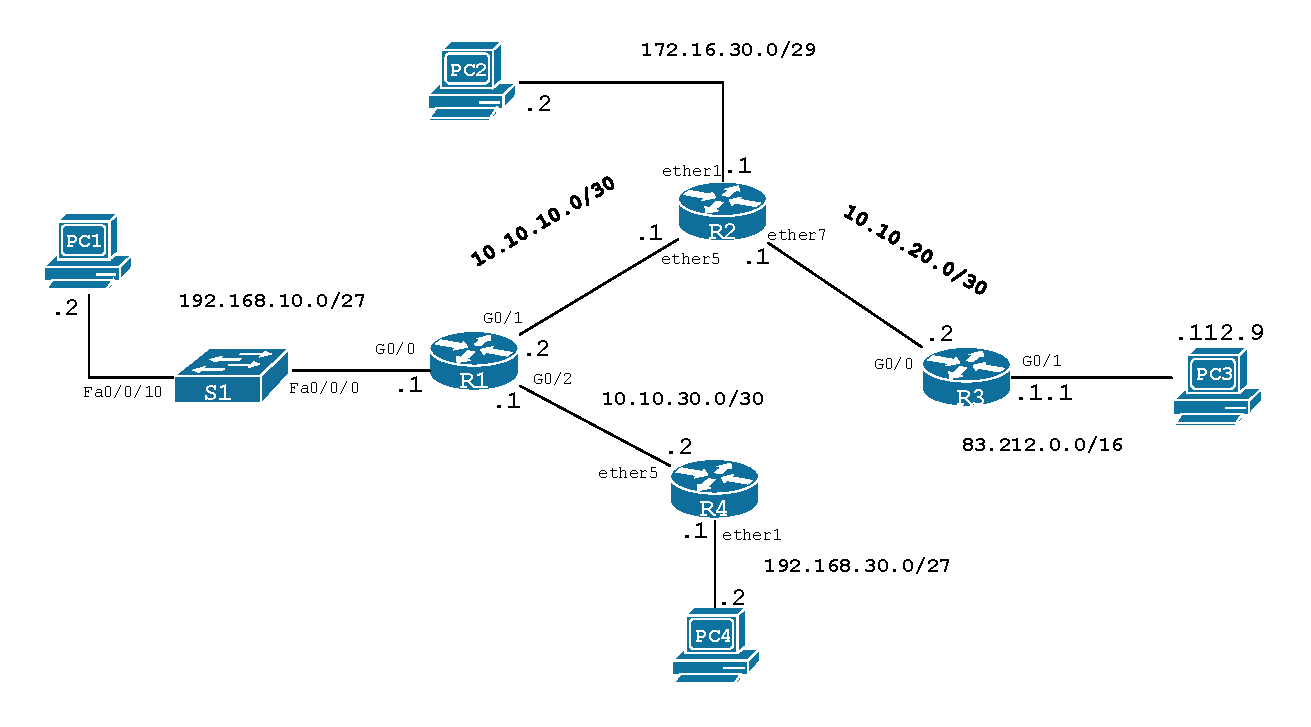
\includegraphics[width=\linewidth]{topology2}
	\caption{Η αναλυτική σχεδίαση της τοπολογίας.}\label{topology2}
\end{figure}

\begin{IpAddressTable}{Σχήμα διευθυνσιοδότησης της τοπολογίας.}{addr}
						& \ip{Loopback0}	& \ip{1.1.1.1}	 	 & \ip{255.255.255.255} & \\
						& \ip{Gi0/0}		& \ip{192.168.10.1}	 & \ip{255.255.255.0} 	& \\
\multirow{-3}{*}{R1}	& \ip{Gi0/1}		& \ip{172.16.1.1}	 & \ip{255.255.255.252} & \multirow{-3}{*}{-}\\
\rowcolor{lightgray}	& \ip{Loopback0}	& \ip{2.2.2.2}	 	 & \ip{255.255.255.255} & \\
\rowcolor{lightgray}	& \ip{Gi0/0}		& \ip{192.168.20.1}	 & \ip{255.255.255.0} 	& \\
\rowcolor{lightgray}
\multirow{-3}{*}{R2}	& \ip{Gi0/1}		& \ip{172.16.1.2}	 & \ip{255.255.255.252} & \multirow{-3}{*}{-}\\
				PC1 	& \NIC	  			& \ip{192.168.10.2}	 & \ip{255.255.255.0} 	& \ip{192.168.10.1}\\
\rowcolor{lightgray}
				PC2		& \NIC	  			& \ip{192.168.20.2}	 & \ip{255.255.255.0} 	& \ip{192.168.20.1}
\end{IpAddressTable}


\section{Υλοποίηση τοπολογίας}

\subsection{Συνδεσμολογία}
Ξεκινώντας την υλοποίηση της τοπολογίας, συνδέστε με καλώδια UTP τους υπολογιστές και τους δρομολογητές, όπως φαίνεται στο σχήμα της τοπολογίας. Προσέξτε να συνδέσετε τα καλώδια στις κατάλληλες διεπαφές των δρομολογητών, σύμφωνα με την αναλυτική σχεδίαση της τοπολογίας που έχετε αποφασίσει να ακολουθήσετε.

\subsection{Παραμετροποίηση δρομολογητών}
Aφού έχετε συνδέσει σωστά τα καλώδια, ξεκινήστε την παραμετροποίηση των δικτυακών συσκευών. Αρχικά, συνδεθείτε μέσω κονσόλας στον δρομολογητή του δικτύου 192.168.10.0/24, μετονομάστε τον σε \textbf{R1} και αναθέστε στη διεπαφή \ip{GigabitEthernet0/0} τη διεύθυνση \ip{192.168.10.1} με μάσκα υποδικτύου την \ip{255.255.255.0}. Για την εφαρμογή αυτών των ρυθμίσεων εκτελέστε τις εντολές που παρατίθενται στον πίνακα \ref{tab:r1}.

\begin{CommandTable*}{Εντολές για την παραμετροποίηση του δρομολογητή \texttt{R1}}{r1}{12cm}{6cm}
	Router>\textbf{enable} & Εισέλθετε σε κατάσταση επαυξημένων δικαιωμάτων.\\
	Router\#\textbf{configure terminal} & Εισέλθετε σε κατάσταση ρυθμίσεων.\\
	Router(config)\#\textbf{hostname R1} & Μετονομάστε τον δρομολογητή σε \texttt{R1}.\\
	R1(config)\#\textbf{interface Gi0/0} & Εισέλθετε στην κατάσταση ρυθμίσεων της διεπαφής \texttt{GigabitEthernet 0/0}.\\
	R1(config-if)\#\textbf{ip address 192.168.10.1 255.255.255.0} & Αναθέστε την επιθυμητή διεύθυνση IP και μάσκα στη διεπαφή.\\
	R1(config-if)\#\textbf{no shutdown} & Ενεργοποιήστε διαχειριστικά τη διεπαφή.\\
	R1(config-if)\#\textbf{exit}& Εξέλθετε από την κατάσταση ρυθμίσεων της συγκεκριμένης διεπαφής.
\end{CommandTable*}

\begin{givecommandbox}
	Με αντίστοιχο τρόπο ρυθμίστε το δίκτυο 172.16.1.0/30 αναθέτοντας στη διεπαφή \ip{Gi0/1} του R1 τη διεύθυνση \ip{172.16.1.1} και μάσκα υποδικτύου την \ip{255.255.255.252}. Ακολουθήστε την αντίστοιχη διαδικασία για τον δεύτερο δρομολογητή, βασιζόμενοι πάντα στο σχήμα διευθυνσιοδότησης.
\end{givecommandbox}

\subsection{Διεπαφές βρόχου}
Οι δρομολογητές διαθέτουν διαφορετική διεύθυνση IP για κάθε διεπαφή που συμμετέχει σε διαφορετικό δίκτυο. Συνεπώς, είναι δύσκολος ο προσδιορισμός ενός δρομολογητή μέσω της διεύθυνσης IP, ειδικά για μεγάλες τοπολογίες, όταν αυτός ανήκει σε πολλά δίκτυα. Γιαυτό, αποτελεί καλή πρακτική ο ορισμός μιας διεύθυνσης βρόχου (loopback address), η οποία  χρησιμοποιείται για τον ευκολότερο προσδιορισμό ενός δρομολογητή. Για παράδειγμα, ο διαχειριστής μπορεί να χρησιμοποιήσει την εν λόγω διεύθυνση για να συνδεθεί με SSH στον δρομολογητή. Ακόμη, η διεύθυνση μπορεί να χρησιμοποιηθεί ως αριθμός ταυτοποίησης σε πλήθος πρωτοκόλλων (OSPF, EIGRP, SNMP κλπ) ή για πειραματικούς σκοπούς, ώστε να προσομοιωθεί ένα εξωτερικό δίκτυο, χωρίς να υπάρχει η αντίστοιχη φυσική διεπαφή.

H διεύθυνση βρόχου αντιστοιχίζεται σε μια διεπαφή βρόχου (loopback interface), η οποία είναι εικονική και υλοποιημένη αποκλειστικά σε λογισμικό. H IANA έχει δεσμεύσει την ομάδα διευθύνσεων 127.0.0.0/8 για τις διεπαφές βρόχου, ωστόσο η χρήση αυτής της ομάδας δεν είναι δεσμευτική για μη παραγωγικά δίκτυα.

Για να δημιουργήσετε μια διεπαφή βρόχου στον R1 δώστε την εντολή που ακολουθεί:

\begin{CommandBox}
R1(config)#`\textbf{interface loopback 0}`
R1(config-if)#
*Aug 24 23:29:42.827: %LINEPROTO-5-UPDOWN: Line protocol on Interface Loopback0, 
changed state to up
R1(config-if)#
\end{CommandBox}

Στη συνέχεια μπορείτε να αναθέσετε την επιθυμητή διεύθυνση IP χωρίς μετά να δώσετε την εντολή\ip{ no shutdown}, αφού η διεπαφή είναι πάντα ενεργοποιημένη.

\begin{CommandBox}
R1(config-if)#`\textbf{ip address 1.1.1.1 255.255.255.255}`
\end{CommandBox}

\begin{givecommandbox}
	Επαναλάβετε τις αντίστοιχες εντολές για τον R2.
\end{givecommandbox}

\subsection{Παραμετροποίηση υπολογιστών}
Αλλάξτε τις ρυθμίσεις IPv4 των PC1 και PC2 για τη διεπαφή που συνδέεται στον δρομολογητή, δίνοντας τις ρυθμίσεις IP που φαίνονται στον πίνακα \ref{tab:addr}. Για περιβάλλον Windows, εκτελέστε την εντολή \ip{ncpa.cpl} από τη γραμμή εντολών των Windows, στο παράθυρο που ανοίγει κάντε δεξί κλικ στο «Ethernet», επιλέξτε «Properties» και στη συνέχεια κάντε κλικ στο «Internet Protocol Version 4 (TCP/IPv4)».

\warningbox{Πριν προχωρήσετε, βεβαιωθείτε ότι οι συνδέσεις σημείου προς σημείο είναι σωστά παραμετροποιημένες. Για παράδειγμα, χρησιμοποιήστε το \texttt{\textbf{ping}} για να επιβεβαιώσετε ότι ο PC1 επικοινωνεί με τον R1, ο R1 με τον R2 και ο PC2 με τον R2.}

\subsection{Τροποποίηση πινάκων δρομολόγησης}

Παρατηρώντας τον πίνακα δρομολόγησης του R1, ο δρομολογητής γνωρίζει μόνο τα δίκτυα με τα οποία είναι απευθείας συνδεδεμένος (172.16.1.0/30, 192.168.10.0/24 και 1.1.1.1/32). Είναι αναμενόμενο ο δρομολογητής R1 να μην γνωρίζει το δίκτυο 192.168.20.0/24 του PC2, αφού αυτό δεν έχει διαφημιστεί από κάποιο πρωτόκολλο δυναμικής δρομολόγησης, ούτε έχει εισαχθεί κάποια στατική καταχώρηση στον πίνακα δρομολόγησης.

\begin{CommandBox}
R1#`\textbf{show ip route | begin Gateway}`
Gateway of last resort is not set

     1.0.0.0/32 is subnetted, 1 subnets
C       1.1.1.1/32 is directly connected, Loopback0
     172.16.0.0/16 is variably subnetted, 2 subnets, 2 masks
C       172.16.1.0/30 is directly connected, GigabitEthernet0/1
L       172.16.1.1/32 is directly connected, GigabitEthernet0/1
     192.168.10.0/24 is variably subnetted, 2 subnets, 2 masks
C       192.168.10.0/24 is directly connected, GigabitEthernet0/0
L       192.168.10.1/32 is directly connected, GigabitEthernet0/0
R1#
\end{CommandBox}

Δεδομένου ότι ο δρομολογητής απορρίπτει τα πακέτα για τα οποία δεν υπάρχει αντίστοιχη καταχώρηση στον πίνακά του, οποιοδήποτε πακέτο έχει ως προορισμό το δίκτυο 192.168.20.0/24 απορρίπτεται από τον R1. Για να επικοινωνήσουν οι PC1 και PC2 θα πρέπει είτε να προστεθούν στατικοί κανόνες στους πίνακες δρομολόγησης των δρομολογητών ή να οριστούν προεπιλεγμένες πύλες δικτύου.

H \textbf{προεπιλεγμένη πύλη} (default gateway) αφορά έναν προορισμό, στον οποίον μια δικτυακή συσκευή προωθεί κάθε πακέτο για το οποίο δεν γνωρίζει που βρίσκεται το δίκτυο προορισμού\footnote{Σε ένα τυπικό οικιακό δίκτυο, όλοι οι υπολογιστές έχουν ως προεπιλεγμένη πύλη τον οικιακό δρομολογητή.}. Στην περίπτωση της τοπολογίας, ο R1 μπορεί να αποκτήσει ως προεπιλεγμένη πύλη τον έτερο δρομολογητή R2, ώστε ο R1 να προωθεί όλα τα πακέτα αγνώστου προορισμού (συμπεριλαμβανομένου του 192.168.20/24) στον R2. Για τον ορισμό του R2 ως προεπιλεγμένη πύλη του R1 δώστε την εντολή \texttt{ip route}:

\begin{CommandBox}
R1(config)#`\textbf{ip route 0.0.0.0 0.0.0.0 172.16.1.2}`
\end{CommandBox}
		
H παραπάνω εντολή ορίζει ως πύλη δικτύου τον 172.16.1.2 (R2), με το δίκτυο 0.0.0.0/0 να αναπαριστά «όλα τα δίκτυα». Αντίστοιχα, θα πρέπει και ο δρομολογητής R2 να αποκτήσει προεπιλεγμένη πύλη τον R1, ώστε η επικοινωνία των δρομολογητών να είναι αμφίδρομη. Από τον R2 δώστε την εξής εντολή:

\begin{CommandBox}
R2(config)#`\textbf{ip route 0.0.0.0 0.0.0.0 172.16.1.1}`
\end{CommandBox}

Πλέον, ο πίνακας δρομολόγησης πρέπει να έχει την εξής μορφή:
 
\begin{CommandBox}
R1#`\textbf{show ip route | begin Gateway}`
`\hl{Gateway of last resort is 172.16.1.2 to network 0.0.0.0}`

     1.0.0.0/32 is subnetted, 1 subnets
C       1.1.1.1/32 is directly connected, Loopback0
     172.16.0.0/16 is variably subnetted, 2 subnets, 2 masks
C       172.16.1.0/30 is directly connected, GigabitEthernet0/1
L       172.16.1.1/32 is directly connected, GigabitEthernet0/1
     192.168.10.0/24 is variably subnetted, 2 subnets, 2 masks
C       192.168.10.0/24 is directly connected, GigabitEthernet0/0
L       192.168.10.1/32 is directly connected, GigabitEthernet0/0
`\hl{S*}`   `\hl{0.0.0.0/0 [1/0] via 172.16.1.2}`
R1#
\end{CommandBox}

\subsection{Δοκιμές συνδεσιμότητας}
Δοκιμάστε τη σύνδεση των δύο υπολογιστών στέλνοντας πακέτα ICMP, με την εντολή \ip{ping}, από το PC1 προς το PC2 και αντίστροφα. Αν το \ip{ping} εκτελέστηκε με επιτυχία, τότε σημαίνει ότι το δίκτυο υλοποιήθηκε σωστά. Αν όχι ακολουθήστε τα βήματα της ενότητας «Αντιμετώπιση προβλημάτων».

\begin{assignmentbox}
	Παραδώστε στιγμιότυπο οθόνης που δείχνει επιτυχή εκτέλεση του ping από το PC1 προς το PC2.
\end{assignmentbox}

\begin{assignmentbox}
	Παραδώστε δυο αρχεία με τις ρυθμίσεις των δρομολογητών R1 και R2 αντίστοιχα.
\end{assignmentbox}

\section{Στατική δρομολόγηση}
Αν και ο ορισμός της προεπιλεγμένης πύλης δικτύου για κάθε δρομολογητή έλυσε το πρόβλημα της επικοινωνίας μεταξύ των απομακρυσμένων δικτύων \ip{192.168.10.0/24} και \ip{192.168.20.0/24}, η λύση αυτή δημιουργεί προβλήματα ως προς την απόδοση των δικτύων.

Πιο συγκεκριμένα, η ρύθμιση προεπιλεγμένης πύλης οδηγεί τους δρομολογητές στο να προωθούν \textbf{όλα} τα πακέτα, για τα οποία ο παραλήπτης δεν περιλαμβάνεται στον πίνακα δρομολόγησης. Μέσα σε αυτό το φορτίο μπορεί να βρίσκονται πακέτα που δεν χρειάζεται να προωθηθούν, όπως πακέτα που προορίζονται για το Διαδίκτυο. Δεδομένης της τοπολογίας που έχει σχεδιαστεί, δεν προβλέπεται επικοινωνία με άλλα δίκτυα, συνεπώς, η προώθηση οποιονδήποτε πακέτων που προορίζονται για δίκτυα εκτός των 192.168.20.0/24 και 172.16.1.0/30 αποτελεί περιττή επιβάρυνση, η οποία μπορεί να αποτραπεί.

Διαπιστώνοντας ότι η ρύθμιση προεπιλεγμένης πύλης δεν είναι ιδανική για τη συγκεκριμένη τοπολογία, θα την αναιρέσετε αντικαθιστώντας την από στατικές διαδρομές για τους δρομολογητές R1 και R2. Πιο συγκεκριμένα, θα πρέπει να γνωστοποιήσετε στον κάθε δρομολογητή την ύπαρξη του απομακρυσμένου δικτύου, δηλαδή να γνωστοποιήσετε στον R1 την ύπαρξη του \ip{192.168.20.0/24} και στον R2 την ύπαρξη του δικτύου \ip{192.168.10.0/24}, ενημερώνοντας κατάλληλα τους πίνακες δρομολόγησης. Η διαδικασία αυτή γίνεται με την εντολή \texttt{ip route}, η οποία συντάσσεται ως εξής: 

\begin{CommandBox}
Router(config)#`\textbf{ip route} \textit{destination-network} \textit{mask} \{\textit{next\_hop} | \textit{interface}\}`
\end{CommandBox}

Όπου \texttt{\textit{destination}} η ταυτότητα του δικτύου προορισμού (network ID), \texttt{\textit{mask}} η μάσκα του δικτύου προορισμού, \texttt{\textit{next\_hop}} η διεύθυνση IP του δρομολογητή επόμενου άλματος (next hop), δηλαδή του «απέναντι» δρομολογητή, και \texttt{\textit{interface}} η διεπαφή από την οποία θα εξέλθει το πακέτο για να φτάσει στον δρομολογητή επόμενου άλματος.

Συμβουλευόμενοι τον πίνακα \ref{tab:static}, αναιρέστε την εντολή προεπιλεγμένης πύλης και προσθέστε την κατάλληλη καταχώρηση στον πίνακα δρομολόγησης για τον R1.

\begin{CommandTable*}{Ορισμός στατικών διαδρομών για τον \texttt{R1}}{static}{11cm}{7cm}
	R1(conf)\#\textbf{no ip route 0.0.0.0 0.0.0.0 172.16.1.2} & Αναιρέστε τον ορισμό προεπιλεγμένης πύλης δικτύου με την εντολή \texttt{no}.\\[0.125cm]
	R1(conf)\#\textbf{ip route 192.168.20.0 255.255.255.0 172.16.1.2} & Ορίστε την στατική καταχώρηση στον πίνακα δρομολόγησης
\end{CommandTable*}

Πλέον, ο πίνακας δρομολόγησης του R1 πρέπει να έχει την εξής μορφή:

\begin{CommandBox}
R1#`\textbf{show ip route | begin Gateway}`
Gateway of last resort is not set

     1.0.0.0/32 is subnetted, 1 subnets
C       1.1.1.1/32 is directly connected, Loopback0
     172.16.0.0/16 is variably subnetted, 2 subnets, 2 masks
C       172.16.1.0/30 is directly connected, GigabitEthernet0/1
L       172.16.1.1/32 is directly connected, GigabitEthernet0/1
     192.168.10.0/24 is variably subnetted, 2 subnets, 2 masks
C       192.168.10.0/24 is directly connected, GigabitEthernet0/0
L       192.168.10.1/32 is directly connected, GigabitEthernet0/0
`\hl{S}`   `\hl{192.168.20.0/24 [1/0] via 172.16.1.2}`
\end{CommandBox}

\begin{givecommandbox}
	Δώστε τις αντίστοιχες εντολές του πίνακα \ref{tab:static} στον R2, ώστε να προσθέσετε στατική διαδρομή για το δίκτυο 192.168.10.0/24 μέσω του R1.
\end{givecommandbox}

Δοκιμάστε πάλι τη συνδεσιμότητα των PC1 και PC2 με πακέτα ICMP και επιβεβαιώστε την σωστή λειτουργία της τοπολογίας.

\begin{assignmentbox}
	Παραδώστε δυο αρχεία με τις ρυθμίσεις των δρομολογητών R1 και R2 αντίστοιχα.
\end{assignmentbox}

\section{Αντιμετώπιση προβλημάτων}
Σε περίπτωση που τα \ip{ping} αποτύχουν, θα πρέπει να πρέπει να προσδιορίσετε το πρόβλημα που υπάρχει και να το επιλύσετε. Μπορείτε να δοκιμάσετε τα εξής:
\begin{itemize}	
	\item Κάντε \ip{ping} μεταξύ του κάθε υπολογιστή και του δρομολογητή του, καθώς και μεταξύ των δυο δρομολογητών, ώστε να προσδιορίσετε αν μια συγκεκριμένη ζεύξη είναι προβληματική.
	
	\item Δοκιμάστε την \ip{tracert} για να διαπιστώσετε αν σταματάτε να λαμβάνετε απόκριση από κάποιο συγκεκριμένο σημείο της τοπολογίας.
	
	\item Ελέγξτε με την εντολή \ip{show ip interface brief} ότι οι διεπαφές που πρέπει να χρησιμοποιηθούν είναι ενεργοποιημένες και έχουν τη σωστή διευθυνσιοδότηση IP. 
	
	\item Επιβεβαιώστε ότι σε κάθε πίνακα δρομολόγησης υπάρχουν οι απαραίτητες καταχωρήσεις με τις σωστές IP και μάσκες, ώστε τα πακέτα να προωθούνται στον προορισμό τους. Μπείτε στη θέση του δρομολογητή και προσπαθήστε, με τα δεδομένα του πίνακα δρομολόγησης που βλέπετε, να αποφανθείτε για τις ενέργειες του δρομολογητή. 
	
	\item Βεβαιωθείτε ότι το τείχος προστασίας των Windows κάθε υπολογιστή είναι απενεργοποιημένο ή ότι υπάρχει κανόνας σε αυτά ώστε να μην απορρίπτονται πακέτα που έρχονται από το τοπικό δίκτυο του έτερου υπολογιστή. 
\end{itemize}

\end{document}